
\ifx\isEmbedded\undefined
\documentclass[12pt]{article}
	
% FONT RELATED
%\usepackage{times} %Move to times font
\usepackage[labelfont=bf,textfont=it]{caption}


% LINKS, PAGE OF CONTENT, REF AND CROSS-REF, HEADERS/FOOTERS
\usepackage{hyperref}
\hypersetup{
    colorlinks,
    citecolor=black,
    filecolor=black,
    linkcolor=black,
    urlcolor=black
}
%\usepackage[breaklinks=true]{hyperref}
\usepackage{fancyhdr}
\usepackage{acronym}

% FIGURES, GRAPHICS, TABLES
\usepackage{graphicx}
\usepackage{parskip}
\usepackage{subfigure}

% COLOURS, TEXT AND FORMATTING
\usepackage{array}
\usepackage{color}
\usepackage{setspace}
\usepackage{longtable}
\usepackage{multirow}

% ADVANCED MATHS, PSEUDO-CODE
\usepackage{amsmath}
\usepackage{alltt}
\usepackage{amsfonts}
\usepackage{listings}
\usepackage{amsmath}

% BIBLIOGRAPHY
\usepackage[authoryear]{natbib}
\bibpunct{(}{)}{;}{a}{}{,}

% USE IN DISSER:

\setlength\oddsidemargin{1.5cm}
\setlength\evensidemargin{5cm}

\setlength\textheight{9.0in}
\setlength\textwidth{5.1in}

% indent at each new paragrapg
\setlength\parindent{0.5cm}

\setlength\topmargin{-0.2in}
\renewcommand{\baselinestretch}{1.3}

%REPORT

%\setlength\oddsidemargin{1cm}
%\setlength\evensidemargin{0.3in}
%%\setlength\headsep{2.5in}
%
%\setlength\textheight{9.0in}
%\setlength\textwidth{5.5in}
%
%% indent at each new paragrapg
%\setlength\parindent{0.5cm}
%
%%\setlength{\parskip}{10.5ex}
%
%\setlength\topmargin{-0.2in}

%\newcommand{\HRule}{\rule{\linewidth}{0.5mm}}
\newcommand{\HRule}{\rule{\linewidth}{0.0mm}}

%% macros
\newcommand{\RR}{\mathbb{R}} 
\newcommand{\pt}[1]{\mathbf{#1}} 

% Color definitions (RGB model)
\definecolor{ms-comment}{rgb}{0.1, 0.4, 0.1}
\definecolor{ms-question}{rgb}{0.8, 0.2, 0.2}
\definecolor{ms-new}{rgb}{0.2, 0.4, 0.8}

\newcommand\red[1]{{\color{red}#1}}
\newcommand\blue[1]{{\color{blue}#1}}
\newcommand\comment[1]{{\iffalse #1 \fi}}

\setcounter{secnumdepth}{3}
\setcounter{tocdepth}{3} 

\graphicspath{{../img/}}
\begin{document}
%\maketitle
\fi

\section{Software System} \label{sec_software}
The algorithms described in the previous section were implemented in C++, using QT, OpenGl and the NGL library. The software takes OBJ files as input data for the piece of cloth and the objects it collides with. The software system and its design are described in the ASE report. To help locate the algorithms, This report includes an annotated class diagram, see image \ref{fig_class}. Since it is hard to read in this size, I included the png file in my submission. While the elements of the modified half edge structure are represented as classes conceptually, they are implemented as structs in the TriangleRenderStructure.h file.\\

\begin{figure}
   \centering
     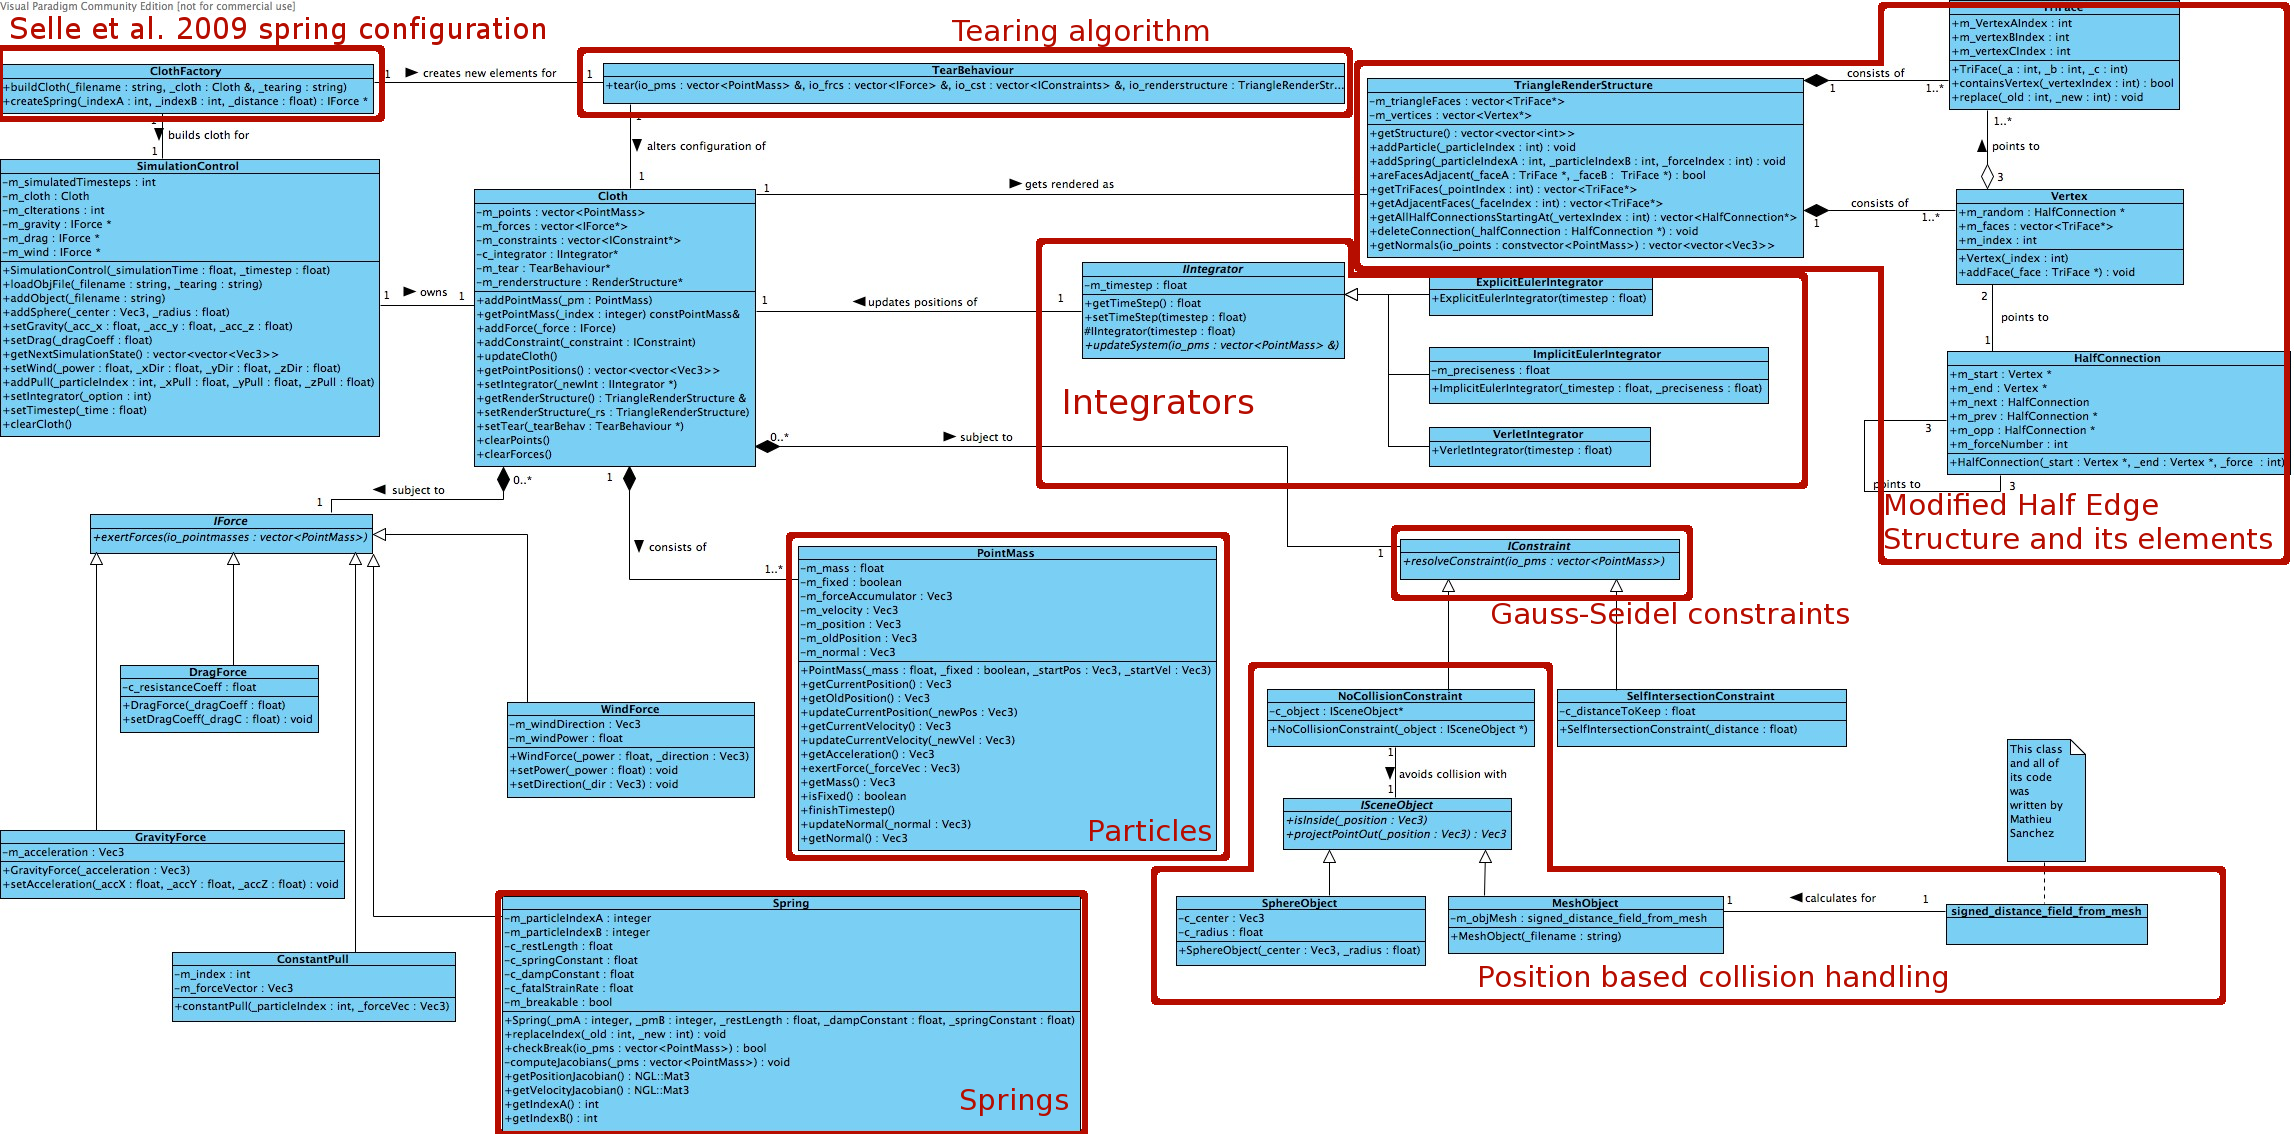
\includegraphics[width=\textheight, angle = 90]{img/annotated_diagram.png}
  \caption{The presented class diagram. The diagrams shows where to find the algorithms described in this report.}
 \label{fig_class}
\end{figure}

\ifx\isEmbedded\undefined
% References
\addcontentsline{toc}{section}{References}
\bibliographystyle{../ref/harvardnat}
\bibliography{../ref/master}
\pagebreak
\end{document}
\fi